\section{Laboratoire de Pulsipher}

\subsection{Jebble}\label{sec:jebble}
\noindent
\includegraphics[width=\linewidth]{_img/places/jebble.png}
\'A l’extrémité de la bordure extérieure, complètement gelée à l’image de Hoth, Jebble constituait autrefois le dernier rempart de défense de la République contre les Mandaloriens. Jebble a été le théâtre des évènements concernant le Talisman de Muur, \nameref{sec:celeste-morne} et \nameref{sec:pulsipher}. C’est durant ces évènements que la planète a été bombardé entièrement par la flotte de \textbf{Cassus Fett} afin d’éviter la contagion des Rakghouls. Ce bombardement a fait fondre les glaces de Jebble et les installations de Pulsipher ont coulé dans les eaux bouillonnantes qui ont regelé par-dessus.

Il y a plus de 1~000~ans des mineurs qui cherchaient à exploiter les ressources de la planète, sont tombés sur les installations de Pulsipher, y ont trouvé l’oubliette de Dreya qu’ils ont vendu en tant que «~Boite de Jebble~».

Depuis la planète Jebble a sombré dans le désintérêt le plus complet pour le reste de la galaxie.

\subsection{Astroport de Kriloo City}
Bon, peu importe où ils choisissent de se poser, ils arrivent ici :p.

Kriloo City est une ville de moyenne ampleur. Comme la plupart des villes de Jebble, elle vie essentiellement de l’exploitation des ressources de la planète, elle est surtout composée de mineurs. On y trouve toutes les institutions habituelles, cantinas, bibliothèques, musés, \ldots

\'A leur arrivée, les héros devront trouver des informations sur Pulsipher et ces installations sous la glace. C’est à la bibliothèque qu’ils trouveront cela. Un jet de \emph{Recherche} dans les archives leur apprendra les quelques évènements de l’histoire de Jebble nécessaire à la localisation du laboratoire. Avec une Relance ils lisent quelque chose sur la «~\nameref{sec:boite-de-jebble}~» mais c’est pas bien clair. Ils peuvent aussi demander à la bibliothécaire, une Besalisk avec 4 paires de bras (très pratique pour organiser les documents). Elle leur raconte la même chose que les archives, leur indique où exactement se situe l’entrée de la veine qui mène aux installations enfouies sous la glace. Elle ne leur parle pas de la boite par contre.

Ils ont ensuite le temps de faire des emplettes pour résister au froid (Manteaux, médipac, \ldots) avant de partir pour le laboratoire. Attention, la température de Jebble oscille entre -12° et -30°. Ce qui signifie que tous les héros qui n’ont pas de résistance particulière au froid feront des jets de Vigueur pendant le scénario. Les héros qui n’ont rien acheté pour se couvrir ajouteront un malus de -2 au malus demandé lors du jet. Chaque échec vaudra un niveau de fatigue (cf les règles du froid dans le bouquin de base).

\subsection{En route}
\noindent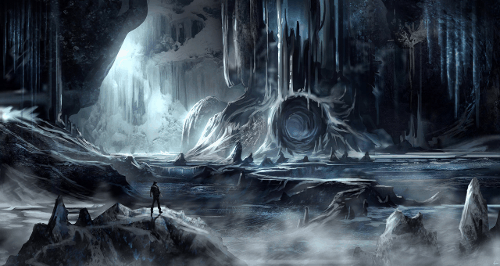
\includegraphics[width=\linewidth]{_img/places/jebble-cave.png}
Nous voilà à l’entrée de la caverne menant aux installations. Avant de s’y engouffrer, tous les héros font un jet de \emph{Vigueur} avec un malus de -2 pour la résistance au froid. En effet, ils ont passé 4 heures à marcher dans la neige par -20° pour arriver jusque-là. Ceux qui ratent prennent un niveau de fatigue.

En entrant dans la grotte, les héros avancent le long d’un étroit tunnel de glace qui s’enfonce dans la glace de l’océan jusqu’à une immense cavité. \'A leur arrivée, des chauves-souries “locale” s’envolent, \ldots bref à vous de décrire. Au fond de la cavité, on distingue des bâtiments pris dans la glace et une entrée creusée à même la glace.

Quand les chauve-souries ont fini de fuir, un grognement se fait entendre dans la grotte et, un \nameref{sec:wampa} surgi de derrière un pilier de glace et s’avance vers eux à grand pas.\\

Une fois le Wampa hors combat, les héros ont le choix de se reposer au près d’un feu pour récupérer de leur fatigue et panser leurs blessures ou d’entrer direct dans le labo.

\subsection{Le laboratoire}

Le laboratoire de Pulsipher possède une IA chargée de sécuriser le laboratoire et d’écarter les intrus. Cette IA, \nameref{sec:lucy-pher} (par ce que ‘\emph{Luc[Puls]ipher}’), est en veille mais les héros vont la réveiller en entrant dans le labo. 

Les héros entrent donc dans le labo de Pulsipher (voir le plan p.~\pageref{sec:plan-labo-pulsipher}). L’entrée est un long sas de plusieurs mètres avant d’arriver dans le laboratoire lui-même. Dans le labo, seuls les sanitaires sont accessibles, tout le reste est verrouillé et doit être soit \textit{Piraté} soit \textit{Forcé}, au choix des héros. Pas de difficulté particulière pour les jets de \textit{Piratage} ou de \textit{Force}, s’ils utilisent un outil approprié pour forcer les portes, ils ont un bonus de +2 au jet de force.

L’ouverture de la première porte déclenche le réveil de Lucy. \'A coté de ce moment il lui faut 5mn (temps IRL) pour sortir de veille et être pleinement activée. Dès que Lucy est activée, le labo se verrouille. Le seul moyen pour les héros de sortir est de débrancher l’ordinateur central.

Lucy dispose de plusieurs moyens pour dissuader les intrus:
\begin{rebelist}
    \item Tous les piratages de portes prennent un malus de -2. Forcer les portes reste possible.
    \item Contrôle environnemental. Lucy peut modifier la température et couper le recyclage de l’air.
    \item Caméras disponibles sur tout le laboratoire (points bleus sur la carte).
    \item Canon Blaster rétractable du plafond (points rouge sur la carte).\\
        \textit{2d10 (1)}
    \item Meute de 5x \nameref{sec:cybercleps}
\end{rebelist}

Donc là les héros sont un peu en galère. La destruction des caméras et Canons dans un secteur rend Lucy aveugle sur le secteur/pièce. Du coup si ça arrive, lâchez les cleps. Sinon laissez les galérer. Les chiens sont là au cas où vos héros s’en sortiraient trop bien. Utilisez-les pour doser la difficulté.\\

Une fois le labo sécurisé, voici la liste des pièces et ce que l’on peut y trouver. Les pièces sont numérotées sur la carte.

\subsubsection{1. Poste Sécurité}
La première pièce à droite en entrant, le PC sécurité, quand il fonctionne donne une vision sur l’ensemble des caméras et des défenses du laboratoire. Il donne un accès au serveur central via un mot de passe. Néanmoins tout y est vieux et obsolète, la moitié des écrans sont brisés les autres clignotent. En mode verrouillage rien n’est accessible depuis ces terminaux.

\subsubsection{2. Salle de pause}
En entrant à gauche, contient des fauteuils des sièges, un distributeur de barres énergétique et de boisson encore rempli. \'A vos héros de voir s’ils se risquent à y goutter. Les barres énergétiques se transforment en poussière à l’ouverture et s’ils gouttent une boisson, ils sont secoués par le goût infâme pendant 10mn.

\subsubsection{3. Débarras}
Un genre de placard de stockage de tout et n’importe quoi. Rien de spécial à y trouver.

\subsubsection{4. Local de contrôle environnemental}
On y gérait toutes les fonctions environnementales de la base. En cas de problème, la base pouvait se verrouiller et devenir autonome. L’air y est recyclé et tempéré depuis les systèmes de ce local. Les serveurs sont indépendants du serveur central mais Lucy peut les commander pour gérer les menaces infectieuses si besoin ou d’autres problèmes de ce genre. Tant que la base n’est pas verrouillée, toutes les commandes sont accessibles. Dès le verrouillage des installations, il faut réussir un \textit{Piratage} pour y parvenir.

\subsubsection{5. Dortoirs}
Les dortoirs des scientifiques du laboratoire. \'A disposition des personnes travaillant dans les installations, ils permettaient de rester dormir ou de se reposer. Les scientifiques n’y habitaient pas à l’année. Rien de spécial à trouver ici non plus.

\subsubsection{6. Garage}
Le garage est une vaste pièce. Il reste un genre de Jeep Rover en bon état mais la batterie est morte et les portes du garage sont condamnés par la glace. On trouve dans le garage divers outils et des pièces de rechange pour véhicules, ainsi que 2 Medipacs.

\subsubsection{7. Laboratoire Principal}
Pièce centrale des installations, c’est ici qu’étaient faites toutes les recherches. Elle est équipée de tout le matériel d’analyse dont un scientifique pouvait rêver \ldots il y a 3~000 ans. Malgré l’age du matériel il reste fonctionnel et la sortie de veille des installations a rétablie l’alimentation. Un \textit{Soin} effectué dans cette pièce avec les appareils présents est accompagné d’un bonus +2 et ne consomme pas de Medipac.

\subsubsection{8. Zone de quarantaine}

\begin{wrapfigure}{r}{0.4\linewidth}
    \vspace{-5\baselineskip}
    \centering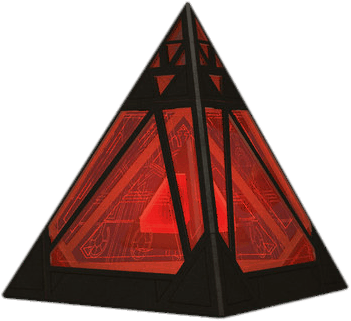
\includegraphics[width=\linewidth]{_img/holocron-sith.png}
    \vspace{-2\baselineskip} 
\end{wrapfigure}
Lieu où étaient stockés les matières dangereuses ou soupçonnées dangereuses. On y trouve un tas de containers étanches, certains ouverts d’autres scellés. Des étagères et des réfrigérateurs qui fonctionnent mais la chaîne du froid n’a certainement pas été respectée.

On trouvera dans cette pièce un Holocron Sith, créé par \nameref{fig:karness-muur} lui-même. Cet holocron est pour l’instant inutilisable. Il faut une affinité avec la Force pour l’ouvrir et un genre de clé mentale. Karness a verrouillé son Holocron pour qu’il ne tombe pas dans les mains de ces ennemis. \'A moins de réussir un jet de \textif{Connaissance (Sith/Jedi)} les joueurs ne voient qu’un objet triangulaire. Ceux qui ont \textit{Vision de Force} ressentent l’émanation obscure de l’objet.

Il n’est pas obligatoire de ramener l’Holocron pour l’instant mais ils en auront besoin plus tard donc ils faudra revenir le chercher s’ils ne le trouvent pas maintenant.

\subsubsection{9. Centre de contrôle}
Un ensemble de terminaux sont disponibles dans cette pièce. Tant que Lucy est active, ils sont tous verrouillé et non Piratable.

\'A partir du moment où Lucy est désactivée, les terminaux donnent accès à toutes les informations du Labo, sans \textit{Piratage}. Deux informations sont importantes~:
\begin{rebelist}
    \item L’\nameref{sec:oubliette-de-dreypa} est la clé pour se débarrasser du Talisman de Muur
    \item L’\nameref{sec:talisman-jebble}
\end{rebelist}

\subsubsection{10. Central Informatique}
Le centre nerveux de Lucy. C’est dans cette pièce que se trouve le seul et unique terminal d’accès au programme de Lucy. Si/Quand les héros parviennent à cette pièce, les \nameref{sec:cybercleps} sont systématiquement lâchés. Un \textit{Piratage} est possible. Un succès désactive Lucy, une \textit{Relance} reboute Lucy et permet de la contrôler pour effectuer plus vite les recherches dont les héros ont besoin.

\'A partir du moment où les héros entrent dans la pièce, une phase de combat commence. Les héros peuvent choisir de repousser les chiens le temps que l’un d’eux parvienne à \textit{Pirater} Lucy. Si c’est le cas, le joueur en question reçoit une carte comme les autres mais à son tour il fait un jet de \textit{Piratage}. Dès que le \textit{Piratage} est réussit les chiens sont hors combat.

\subsubsection{Canons \& Caméras}
Sur le \nameref{sec:plan-labo-pulsipher} sont disposé les Caméras (triangles verts) et les tours de canons (carrés rouges). Les caméras sont rotatives. Tous ce qui n’est pas dans le champ d’une caméra n’est pas visible par Lucy.

Les canons aussi sont rotatifs, ils possèdent les caractéristiques de \textit{Canon blaster embarqué}~:
\begin{itemtable}[ X c c c c ]
    \textbf{Type} & \textbf{Porté} & \textbf{Dégâts} & \textbf{Résistance} \\
    Canon blaster & 600            & 2d10  (1)       & 10 \\
\end{itemtable}

\onecolumn
\subsection{Plan du labo de Pulsipher}\label{sec:plan-labo-pulsipher}
\begin{figure}[!h]
	\centering	
	\begin{tikzpicture}[overlay, anchor=north]
		\node at (0,0) {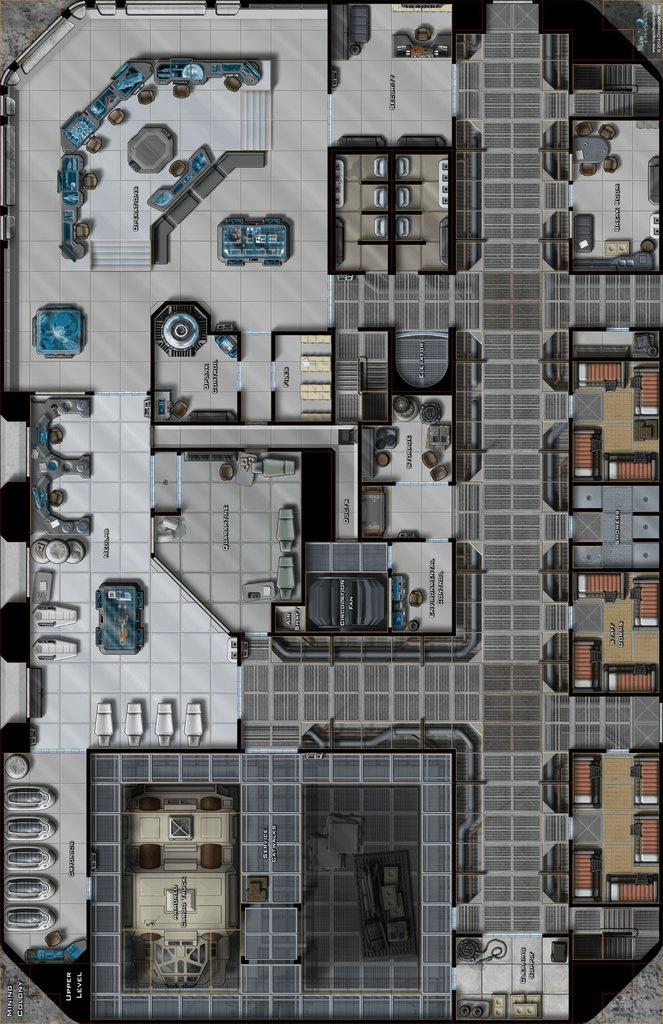
\includegraphics[height=0.94\textheight]{_img/places/labo-pulsipher-map.png}};
		\node at (0,-0.4) {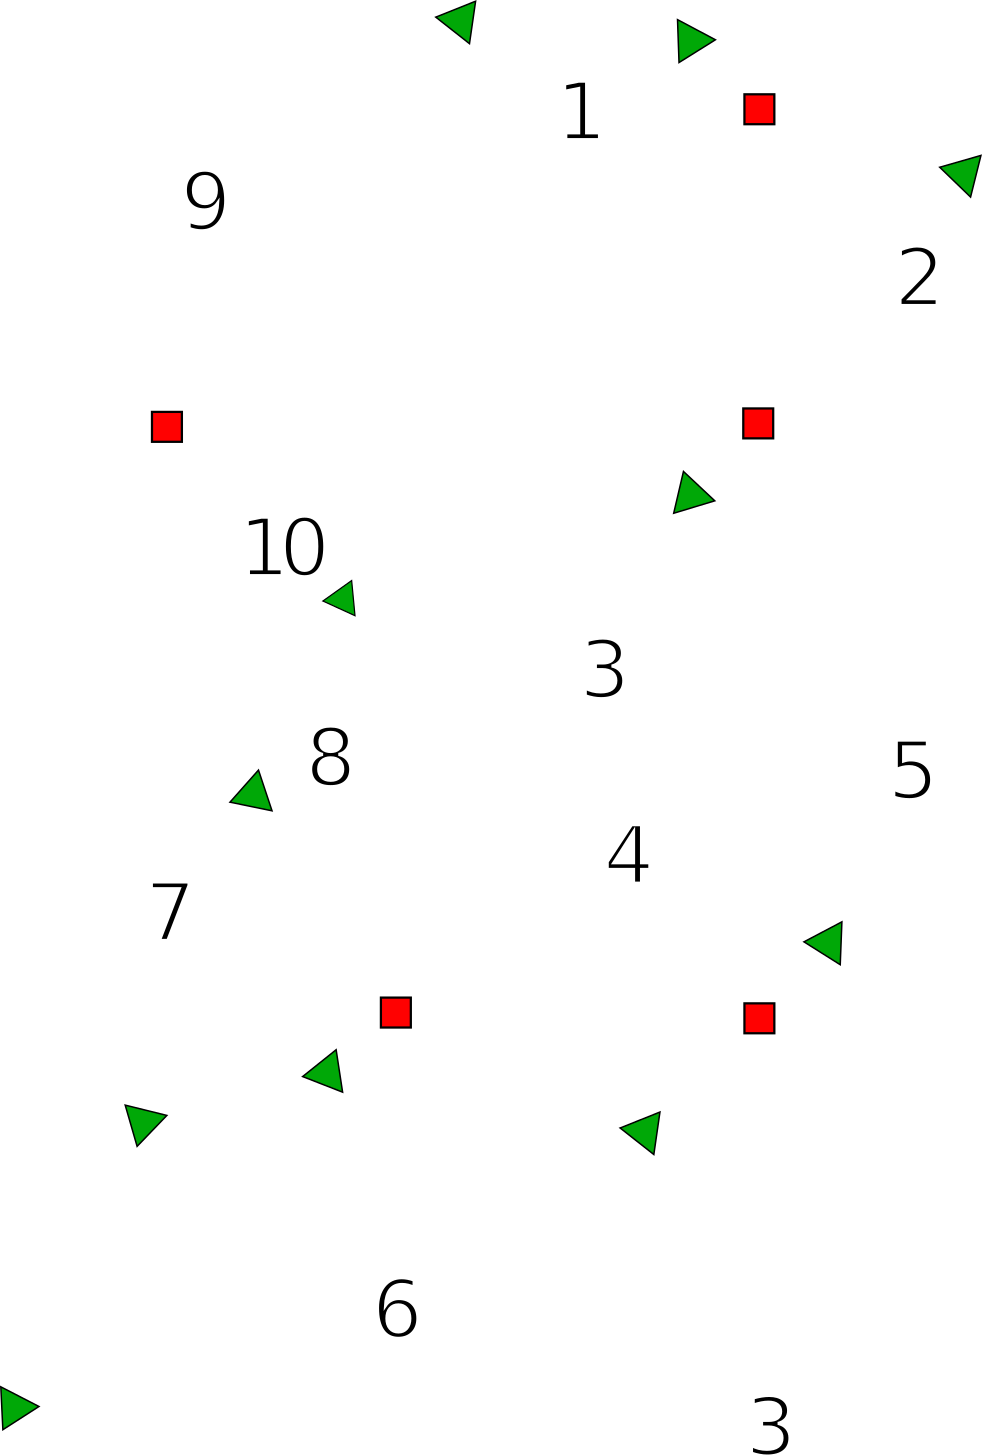
\includegraphics[height=0.89\textheight]{_img/places/labo-pulsipher-layers.png}};
	\end{tikzpicture}
\end{figure}

\twocolumn

\subsection{Oubliette de Dreypa}\label{sec:oubliette-de-dreypa}
Au début de l'Empire Sith, un Seigneur Sith du nom de Lord Dreypa créa, probablement grâce à la sorcellerie sith, une oubliette. Celle-ci avait la capacité de plonger son occupant dans une forme de stase tout en le maintenant conscient et en le soumettant à des tortures. Dreypa la destinait à son rival, le Seigneur Sith Karness Muur, mais ne put jamais mener son projet à terme, du moins de son vivant… 

\subsection{Histoire du Talisman sur Jebble}\label{sec:talisman-jebble}
Les données trouvées dans les ordinateurs du labo apprennent aux héros que \nameref{sec:pulsipher} a voulu s’emparer du pouvoir du Talisman pour créer son propre clan Mandalorien. Mais le Talisman a sa propre conscience, celle de \nameref{fig:karness-muur}. Et son but à lui est de trouver un hôte dont la sensibilité à la Force est le plus élevé possible. Il quitta donc Pulsipher pour s’emparer de \nameref{sec:celeste-morne}, une Jedi venu arrêter les agissements de Pulsipher.

Céleste parvint à se maîtriser juste assez longtemps pour permettre à \textbf{Zayne}, son Padawan, de l’enfermer dans l’\nameref{sec:oubliette-de-dreypa} le temps que ce dernier trouve une solution pour la débarrasser du Talisman. Malheureusement pour eux, c’est à ce moment que \textbf{Cassus Feth} un chef Mandalorien de l’époque, bombarda toute la zone du Labo afin d’endiguer la maladie des rakghouls. Les glaces autour du labo fondirent et engloutirent le Labo et l’oubliette avant de regeler par-dessus.

La population locale connaissait l’oubliette sous le nom \testbf{Boite de Jebble}\ldots 

C’est là que s’arrête les données de l’ordinateur.

\subsection{La Boite de Jebble}\label{sec:boite-de-jebble}
Si nos héros retournent à Kriloo City, et qu’ils posent des questions sur la \textbf{Boite de Jebble}, n’importe qui leur parlera de la légende. Légende qui date d’au moins 1~500~ans. Une boite trouvée 1~km sous la glace, impossible à ouvrir, impossible à scanner, qui a été étudié plusieurs années sans le moindre résultat et qui a fini par être vendu à on ne sait plus qui. On dit que seul un Jedi pourrait l’ouvrir mais il y a un prix à payer. C’est la boite de Pandore version Jebble !

\subsection{\’Epilogue}
Nos héros n’en apprendront pas plus sur Jebble. Ils doivent maintenant se mettre à la recherche de la \textbf{Boite de Jebble}. Pour faciliter la transition avec le prochain scénar, à leur retour au Nimbus, les héros reçoivent un message de leur faction (Alliance ou Empire) leur demandant où ils en sont de leur recherche.

\subsection{Progression}
Toujours à titre indicatif, ce scenario était un peu moins velu que le précédent, c’est seulement \textbf{2~XP} que je distribue aux joueurs s’ils ont trouvé l’Holocron, sinon c’est moitié moins.

